\documentclass[10pt,a4paper]{article}
\usepackage[latin1]{inputenc}
\usepackage{amsmath}
\usepackage{amsfonts}
\usepackage{amssymb}
\usepackage{graphicx}
\usepackage{tikz}
\usepackage{tikz-qtree}
\title{Bioinformatics Summative - Question 2}
\begin{document}
	\begin{center}
		Step 1
		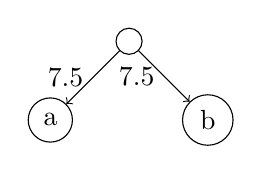
\begin{tikzpicture}
			
			\node[shape=circle, draw=black] (a) at (0,0) {a};
			\node[shape=circle, draw=black] (b) at (2,0) {b};
			\node[shape=circle, draw=black] (ab) at (1,1) {};
			
			\path [->] (ab) edge node[left] {$7.5$} (a);
			\path [->] (ab) edge node[left] {$7.5$} (b);	
		\end{tikzpicture}
		
		\noindent\makebox[\linewidth]{\rule{\paperwidth}{0.4pt}}
		
		Step 2	
		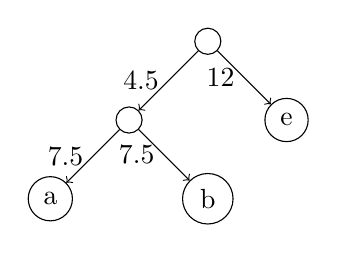
\begin{tikzpicture}
			\node[shape=circle, draw=black] (a) at (0,0) {a};
			\node[shape=circle, draw=black] (b) at (2,0) {b};
			\node[shape=circle, draw=black] (e) at (3.0,1) {e};
			\node[shape=circle, draw=black] (ab) at (1,1) {};
			\node[shape=circle, draw=black] (abe) at (2,2) {};
			
			\path [->] (abe) edge node[left] {$4.5$} (ab);
			\path [->] (abe) edge node[left] {$12$} (e);
			\path [->] (ab) edge node[left] {$7.5$} (a);
			\path [->] (ab) edge node[left] {$7.5$} (b);	
		\end{tikzpicture}

		\noindent\makebox[\linewidth]{\rule{\paperwidth}{0.4pt}}
	
		Step 3
		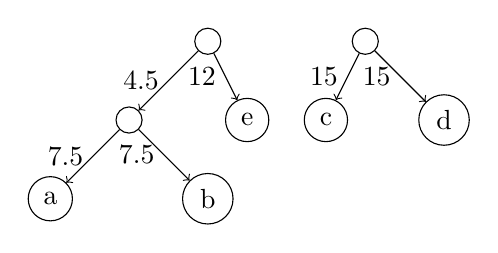
\begin{tikzpicture}
			\node[shape=circle, draw=black] (a) at (0,0) {a};
			\node[shape=circle, draw=black] (b) at (2,0) {b};
			\node[shape=circle, draw=black] (c) at (3.5,1) {c};
			\node[shape=circle, draw=black] (d) at (5,1) {d};
			\node[shape=circle, draw=black] (e) at (2.5,1) {e};
			\node[shape=circle, draw=black] (ab) at (1,1) {};
			\node[shape=circle, draw=black] (abe) at (2,2) {};
			\node[shape=circle, draw=black] (cd) at (4,2) {};
			
			\path [->] (cd) edge node[left] {$15$} (c);
			\path [->] (cd) edge node[left] {$15$} (d);
			\path [->] (abe) edge node[left] {$4.5$} (ab);
			\path [->] (abe) edge node[left] {$12$} (e);
			\path [->] (ab) edge node[left] {$7.5$} (a);
			\path [->] (ab) edge node[left] {$7.5$} (b);	
		\end{tikzpicture}
	
		\noindent\makebox[\linewidth]{\rule{\paperwidth}{0.4pt}}
		
		Step 4
		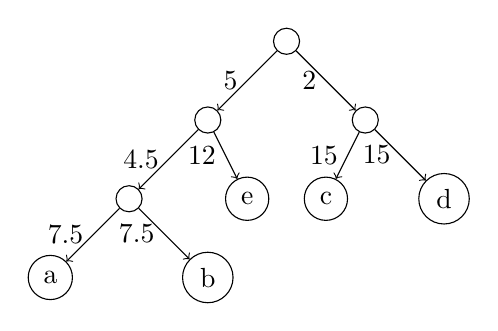
\begin{tikzpicture}
			\node[shape=circle, draw=black] (a) at (0,0) {a};
			\node[shape=circle, draw=black] (b) at (2,0) {b};
			\node[shape=circle, draw=black] (c) at (3.5,1) {c};
			\node[shape=circle, draw=black] (d) at (5,1) {d};
			\node[shape=circle, draw=black] (e) at (2.5,1) {e};
			\node[shape=circle, draw=black] (ab) at (1,1) {};
			\node[shape=circle, draw=black] (abe) at (2,2) {};
			\node[shape=circle, draw=black] (cd) at (4,2) {};
			\node[shape=circle, draw=black] (abecd) at (3,3) {};
			
			\path [->] (abecd) edge node[left] {$5$} (abe);
			\path [->] (abecd) edge node[left] {$2$} (cd);
			\path [->] (cd) edge node[left] {$15$} (c);
			\path [->] (cd) edge node[left] {$15$} (d);
			\path [->] (abe) edge node[left] {$4.5$} (ab);
			\path [->] (abe) edge node[left] {$12$} (e);
			\path [->] (ab) edge node[left] {$7.5$} (a);
			\path [->] (ab) edge node[left] {$7.5$} (b);	
		\end{tikzpicture}
		
		\noindent\makebox[\linewidth]{\rule{\paperwidth}{0.4pt}}
	
		Step 5
		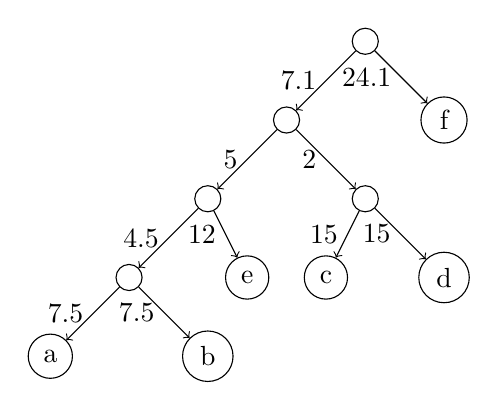
\begin{tikzpicture}
			\node[shape=circle, draw=black] (a) at (0,0) {a};
			\node[shape=circle, draw=black] (b) at (2,0) {b};
			\node[shape=circle, draw=black] (c) at (3.5,1) {c};
			\node[shape=circle, draw=black] (d) at (5,1) {d};
			\node[shape=circle, draw=black] (e) at (2.5,1) {e};
			\node[shape=circle, draw=black] (f) at (5,3) {f};
			\node[shape=circle, draw=black] (ab) at (1,1) {};
			\node[shape=circle, draw=black] (abe) at (2,2) {};
			\node[shape=circle, draw=black] (cd) at (4,2) {};
			\node[shape=circle, draw=black] (abecd) at (3,3) {};
			\node[shape=circle, draw=black] (abecdf) at (4,4) {};
			
			\path [->] (abecdf) edge node[left] {$24.1$} (f);
			\path [->] (abecdf) edge node[left] {$7.1$} (abecd);
			\path [->] (abecd) edge node[left] {$5$} (abe);
			\path [->] (abecd) edge node[left] {$2$} (cd);
			\path [->] (cd) edge node[left] {$15$} (c);
			\path [->] (cd) edge node[left] {$15$} (d);
			\path [->] (abe) edge node[left] {$4.5$} (ab);
			\path [->] (abe) edge node[left] {$12$} (e);
			\path [->] (ab) edge node[left] {$7.5$} (a);
			\path [->] (ab) edge node[left] {$7.5$} (b);	
		\end{tikzpicture}
		
		\noindent\makebox[\linewidth]{\rule{\paperwidth}{0.4pt}}	
	\end{center}

	\pagebreak
	
	\begin{center}
		Step 0
		\[\begin{bmatrix}
			- & a & b & c & d & e & f \\
			a & 0 & 15 & 24 & 29 & 25 & 37\\
			b &  & 0 & 32 & 31 & 23 & 43\\
			c &  &  & 0 & 30 & 43 & 49\\
			d &  &  &  & 0 & 45 & 57\\
			e &  &  &  &  & 0 & 55\\
			f &  &  &  &  &  & 0
		\end{bmatrix}\]
		
		\noindent\makebox[\linewidth]{\rule{\paperwidth}{0.4pt}}
		
		Step 1
		\[\begin{bmatrix}
		- & ab & c & d & e & f \\
		ab & 0 & 28 & 30 & 24 & 40\\
		c &  & 0 & 30 & 43 & 49\\
		d &  &  & 0 & 45 & 57\\
		e &  &  &  & 0 & 55\\
		f &  &  &  &  & 0
		\end{bmatrix}\]
		
		\noindent\makebox[\linewidth]{\rule{\paperwidth}{0.4pt}}
		
		Step 2 
		\[\begin{bmatrix}
		- & abe & c & d & f \\
		abe & 0 & 33 & 35 & 45\\
		c &  & 0 & 30 & 49\\
		d &  &  & 0 & 57\\
		f &  &  &  & 0
		\end{bmatrix}\]

		\noindent\makebox[\linewidth]{\rule{\paperwidth}{0.4pt}}
		
		Step 3 
		\[\begin{bmatrix}
		- & abe & cd & f \\
		abe & 0 & 34 & 45\\
		cd &  & 0 & 53\\
		f &  & & 0
		\end{bmatrix}\]
		
		\noindent\makebox[\linewidth]{\rule{\paperwidth}{0.4pt}}
		
		Step 4
		\[\begin{bmatrix}
		- & abecd & f \\
		abecd & 0 & 48.2\\
		f &  & 0
		\end{bmatrix}\]
		
		\noindent\makebox[\linewidth]{\rule{\paperwidth}{0.4pt}}

	\end{center}
\end{document}